\documentclass[journal,12pt,twocolumn]{IEEEtran}

\usepackage{setspace}
\usepackage{gensymb}
\singlespacing
\usepackage[cmex10]{amsmath}

\usepackage{amsthm}

\usepackage{mathrsfs}
\usepackage{txfonts}
\usepackage{stfloats}
\usepackage{bm}
\usepackage{cite}
\usepackage{cases}
\usepackage{subfig}

\usepackage{longtable}
\usepackage{multirow}

\usepackage{enumitem}
\usepackage{mathtools}
\usepackage{steinmetz}
\usepackage{tikz}
\usepackage{circuitikz}
\usepackage{verbatim}
\usepackage{tfrupee}
\usepackage[breaklinks=true]{hyperref}
\usepackage{graphicx}
\usepackage{tkz-euclide}

\usetikzlibrary{calc,math}
\usepackage{listings}
    \usepackage{color}                                            %%
    \usepackage{array}                                            %%
    \usepackage{longtable}                                        %%
    \usepackage{calc}                                             %%
    \usepackage{multirow}                                         %%
    \usepackage{hhline}                                           %%
    \usepackage{ifthen}                                           %%
    \usepackage{lscape}     
\usepackage{multicol}
\usepackage{chngcntr}

\DeclareMathOperator*{\Res}{Res}

\renewcommand\thesection{\arabic{section}}
\renewcommand\thesubsection{\thesection.\arabic{subsection}}
\renewcommand\thesubsubsection{\thesubsection.\arabic{subsubsection}}

\renewcommand\thesectiondis{\arabic{section}}
\renewcommand\thesubsectiondis{\thesectiondis.\arabic{subsection}}
\renewcommand\thesubsubsectiondis{\thesubsectiondis.\arabic{subsubsection}}

\newtheorem{theorem}{Theorem}
\hyphenation{op-tical net-works semi-conduc-tor}
\def\inputGnumericTable{}                                 %%

\lstset{
%language=C,
frame=single, 
breaklines=true,
columns=fullflexible
}
\begin{document}

\newcommand{\BEQA}{\begin{eqnarray}}
\newcommand{\EEQA}{\end{eqnarray}}
\newcommand{\define}{\stackrel{\triangle}{=}}
\bibliographystyle{IEEEtran}
\raggedbottom
\setlength{\parindent}{0pt}
\providecommand{\mbf}{\mathbf}
\providecommand{\pr}[1]{\ensuremath{\Pr\left(#1\right)}}
\providecommand{\qfunc}[1]{\ensuremath{Q\left(#1\right)}}
\providecommand{\sbrak}[1]{\ensuremath{{}\left[#1\right]}}
\providecommand{\lsbrak}[1]{\ensuremath{{}\left[#1\right.}}
\providecommand{\rsbrak}[1]{\ensuremath{{}\left.#1\right]}}
\providecommand{\brak}[1]{\ensuremath{\left(#1\right)}}
\providecommand{\lbrak}[1]{\ensuremath{\left(#1\right.}}
\providecommand{\rbrak}[1]{\ensuremath{\left.#1\right)}}
\providecommand{\cbrak}[1]{\ensuremath{\left\{#1\right\}}}
\providecommand{\lcbrak}[1]{\ensuremath{\left\{#1\right.}}
\providecommand{\rcbrak}[1]{\ensuremath{\left.#1\right\}}}
\theoremstyle{remark}
\newtheorem{rem}{Remark}
\newcommand{\sgn}{\mathop{\mathrm{sgn}}}
\providecommand{\abs}[1]{\vert#1\vert}
\providecommand{\res}[1]{\Res\displaylimits_{#1}} 
\providecommand{\norm}[1]{\lVert#1\rVert}
%\providecommand{\norm}[1]{\lVert#1\rVert}
\providecommand{\mtx}[1]{\mathbf{#1}}
\providecommand{\mean}[1]{E[ #1 ]}
\providecommand{\fourier}{\overset{\mathcal{F}}{ \rightleftharpoons}}
%\providecommand{\hilbert}{\overset{\mathcal{H}}{ \rightleftharpoons}}
\providecommand{\system}{\overset{\mathcal{H}}{ \longleftrightarrow}}
	%\newcommand{\solution}[2]{\textbf{Solution:}{#1}}
\newcommand{\solution}{\noindent \textbf{Solution: }}
\newcommand{\cosec}{\,\text{cosec}\,}
\providecommand{\dec}[2]{\ensuremath{\overset{#1}{\underset{#2}{\gtrless}}}}
\newcommand{\myvec}[1]{\ensuremath{\begin{pmatrix}#1\end{pmatrix}}}
\newcommand{\mydet}[1]{\ensuremath{\begin{vmatrix}#1\end{vmatrix}}}
\numberwithin{equation}{subsection}
\makeatletter
\@addtoreset{figure}{problem}
\makeatother
\let\StandardTheFigure\thefigure
\let\vec\mathbf
\renewcommand{\thefigure}{\theproblem}
\def\putbox#1#2#3{\makebox[0in][l]{\makebox[#1][l]{}\raisebox{\baselineskip}[0in][0in]{\raisebox{#2}[0in][0in]{#3}}}}
     \def\rightbox#1{\makebox[0in][r]{#1}}
     \def\centbox#1{\makebox[0in]{#1}}
     \def\topbox#1{\raisebox{-\baselineskip}[0in][0in]{#1}}
     \def\midbox#1{\raisebox{-0.5\baselineskip}[0in][0in]{#1}}
\vspace{3cm}
\title{GATE Assignment}
\author{Digjoy Nandi - AI20BTECH11007}
\maketitle
\newpage
\bigskip
\renewcommand{\thefigure}{\theenumi}
\renewcommand{\thetable}{\theenumi}
Download all python codes from 
\begin{lstlisting}
https://github.com/Digjoy12/Signal-Processing/blob/main/Assignment%202-GATE/Codes/code.py
\end{lstlisting}
%
and latex codes from 
%
\begin{lstlisting}
https://github.com/Digjoy12/Signal-Processing/blob/main/Assignment%202-GATE/main.tex
\end{lstlisting}
\section*{\textbf{Problem}}
\textbf{(GATE EC 2020 - Q52)} X($\omega$) is the Fourier Transform of x(t) shown below. The value of $\displaystyle\int\limits_{-\infty}^{\infty} \abs{X(\omega)}^2 d\omega$ (\textbf{rounded off to two decimal places}) is $..................$
\begin{figure}[!ht]
\centering
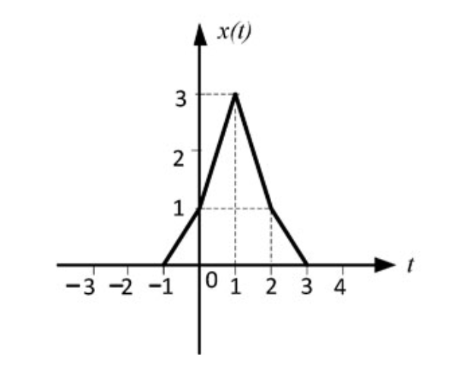
\includegraphics[width=\columnwidth]{plot.png}
\end{figure}

\section*{\textbf{Solution}}
\begin{theorem}[Parseval's energy theorem]
\begin{equation}
    \displaystyle\int\limits_{-\infty}^{\infty} \abs{x(t)}^2 dt &= \cfrac{1}{2\pi}\displaystyle\int\limits_{-\infty}^{\infty} \abs{X(\omega)}^2 d\omega\\
\end{equation}
where $X(\omega)=F_{(\omega)}\{x(t)\}$ represents the continuous Fourier transform of x(t) and $\omega = 2\pi f$  is frequency in radians per second.
\end{theorem}
\begin{proof}
The inverse Fourier Transform of x(t) is
\begin{equation}
    x(t) = \cfrac{1}{2\pi}\displaystyle\int\limits_{-\infty}^{\infty} X(\omega)\exp{(\omega t)} d\omega
\end{equation}
Taking the conjugate of x(t), we get
\begin{equation}
    x^{*}(t) = \cfrac{1}{2\pi}\displaystyle\int\limits_{-\infty}^{\infty} X^{*}(\omega)\exp{(-\omega t)} d\omega
\end{equation}
We know that, total energy of signal x(t) is
\begin{align}
    E_{x(t)}&=\displaystyle\int\limits_{-\infty}^{\infty} \abs{x(t)}^2 dt\\
    &= \displaystyle\int\limits_{-\infty}^{\infty} x(t)x^{*}(t) dt\\
    &= \displaystyle\int\limits_{-\infty}^{\infty} x(t)\Bigg[\cfrac{1}{2\pi}\displaystyle\int\limits_{-\infty}^{\infty} X^{*}(\omega)\exp{(-\omega t)} d\omega\Bigg]dt\\
    &= \cfrac{1}{2\pi}\displaystyle\int\limits_{-\infty}^{\infty}X^{*}(\omega)\displaystyle\int\limits_{-\infty}^{\infty} x(t)\exp{(\omega t)} d\omega\\
    &= \cfrac{1}{2\pi}\displaystyle\int\limits_{-\infty}^{\infty}X^{*}(\omega)X(\omega)\\
    &= \cfrac{1}{2\pi}\displaystyle\int\limits_{-\infty}^{\infty} \abs{X(\omega)}^2 d\omega
\end{align}
\end{proof}
Now, by Parseval's theorem, we know that
\begin{align}
\displaystyle\int\limits_{-\infty}^{\infty} \abs{x(t)}^2 dt &= \cfrac{1}{2\pi}\displaystyle\int\limits_{-\infty}^{\infty} \abs{X(\omega)}^2 d\omega\\
\implies 2\pi \displaystyle\int\limits_{-\infty}^{\infty} \abs{x(t)}^2 dt &= \displaystyle\int\limits_{-\infty}^{\infty} \abs{X(\omega)}^2 d\omega\\
\implies 2\pi \displaystyle\int\limits_{-\infty}^{\infty} {x(t)}^2 dt &= \displaystyle\int\limits_{-\infty}^{\infty} \abs{X(\omega)}^2 d\omega
%\text{Since, x(t) is real}
\end{align}
[\textit{Since, x(t) is real}]\\

Since, shifting of a signal does not change the energy of the signal, therefore left shifting the signal by 1, we get the signal as y(t) = x(t+1)

\begin{figure}[!ht]
\centering
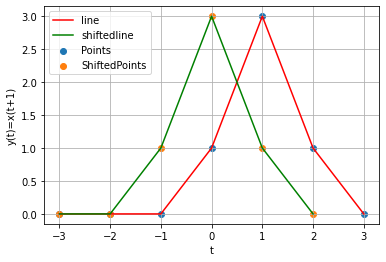
\includegraphics[width=\columnwidth]{download.png}
\caption{Graphical Transformation}
\end{figure}

Now, y(t) is an even function since it is symmetric around the origin.\\
Therefore $y^2(t)$ is also an even signal.\\

\begin{align}
  \displaystyle\int\limits_{-\infty}^{\infty} \abs{X(\omega)}^2 d\omega &= 2\pi \displaystyle\int\limits_{-\infty}^{\infty} {y(t)}^2 dt\\
  &= 4\pi \displaystyle\int\limits_{0}^{\infty} {y(t)}^2 dt\\
  &= 4\pi \left[ \displaystyle\int\limits_{0}^{1} {y(t)}^2 dt +  \displaystyle\int\limits_{1}^{2} {y(t)}^2 dt\right]
\end{align}

For t=0 to t=1,\\
$$y(t) = x(t+1) = -2t + 3$$

For t=1 to t=2, \\
$$y(t) = x(t+1) = -t + 2$$

Therefore,\\

\begin{align}
  \displaystyle\int\limits_{-\infty}^{\infty} \abs{X(\omega)}^2 d\omega &= 4\pi \left[ \displaystyle\int\limits_{0}^{1} {y(t)}^2 dt +  \displaystyle\int\limits_{1}^{2} {y(t)}^2 dt\right]\\
  &= 4\pi \left[ \displaystyle\int\limits_{0}^{1} {(-2t+3)}^2 dt+  \displaystyle\int\limits_{1}^{2} {(-t+2)}^2 dt\right]\\
  &= 4\pi \Bigg[ \displaystyle\int\limits_{0}^{1} {(4t^2 - 12t +9)} dt + \nonumber \\ 
  & \displaystyle\int\limits_{1}^{2} {(t^2 - 4t + 4)} dt\Bigg]\\
  &= 4\pi \left[\cbrak{\cfrac{4t^3}{3}-6t^2+9t}_{0}^{1} +\noumber \\
  & \cbrak{\cfrac{t^3}{3}-2t^2+4t}_{1}^{2}\right]\\
  &= 4\pi \left[\cfrac{13}{3}+\cfrac{1}{3}\right]\\
  &= 4\pi \left[\cfrac{14}{3}\right]\\
  &= 58.61\%
\end{align}

Hence,
$$ \displaystyle\int\limits_{-\infty}^{\infty} \abs{X(\omega)}^2 d\omega = \textbf{58.61\%}$$
\end{document}
